\chapter{Конструкторская часть}

\section{Схема алгоритма Левенштейна}

На рисунках \ref{img:levenshtein_matrix} и \ref{img:levenshtein_recursive} приведены схемы итеративного и рекурсивного алгоритма Левенштейна.


\section{Схема алгоритма Дамерау — Левенштейна}

На рисунке \ref{img:levenshtein_damerau} представлен итеративный алгоритм Дамерау — Левенштейна.

\section*{Вывод}

На основе теоретических данных, полученных из аналитического раздела были построены схемы требуемых алгоритмов.

% don't look at me

% alright

\img{95mm}{levenshtein_detail_set_current_min_distance}{Схема процедуры, вычисляющей текущее расстояние}

\img{250mm}{levenshtein_matrix}{Схема итеративного алгоритма Левенштейна}

\img{105mm}{levenshtein_detail_initial_matrix}{Схема функции, создающей матрицу с инициализированными первой строкой и первым столбцом}

\img{115mm}{levenshtein_detail_init_second_layer}{Схема процедуры, инициализирующей вторую строку и второй столбец}


\begin{figure}[h]
	\center{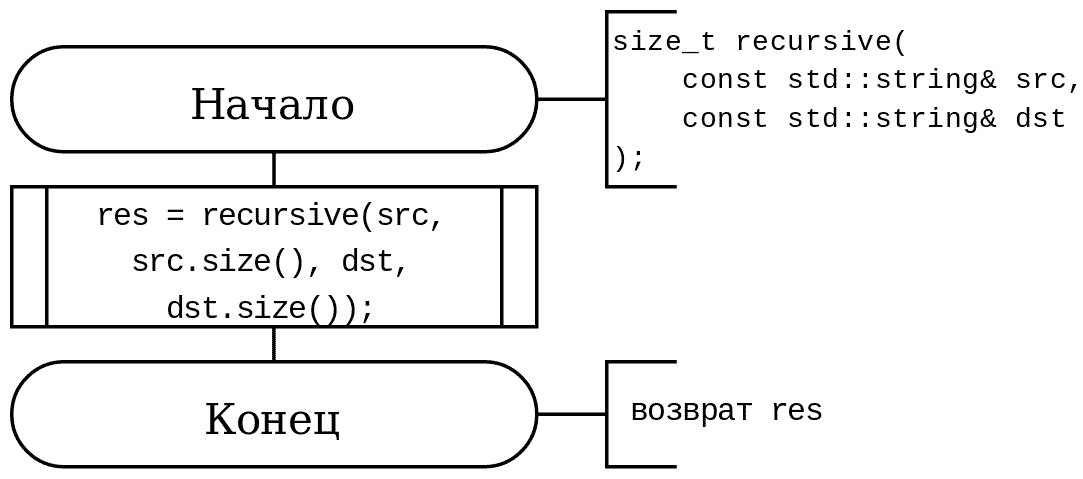
\includegraphics[height=60mm]{inc/img/levenshtein_recursive}}
	\center{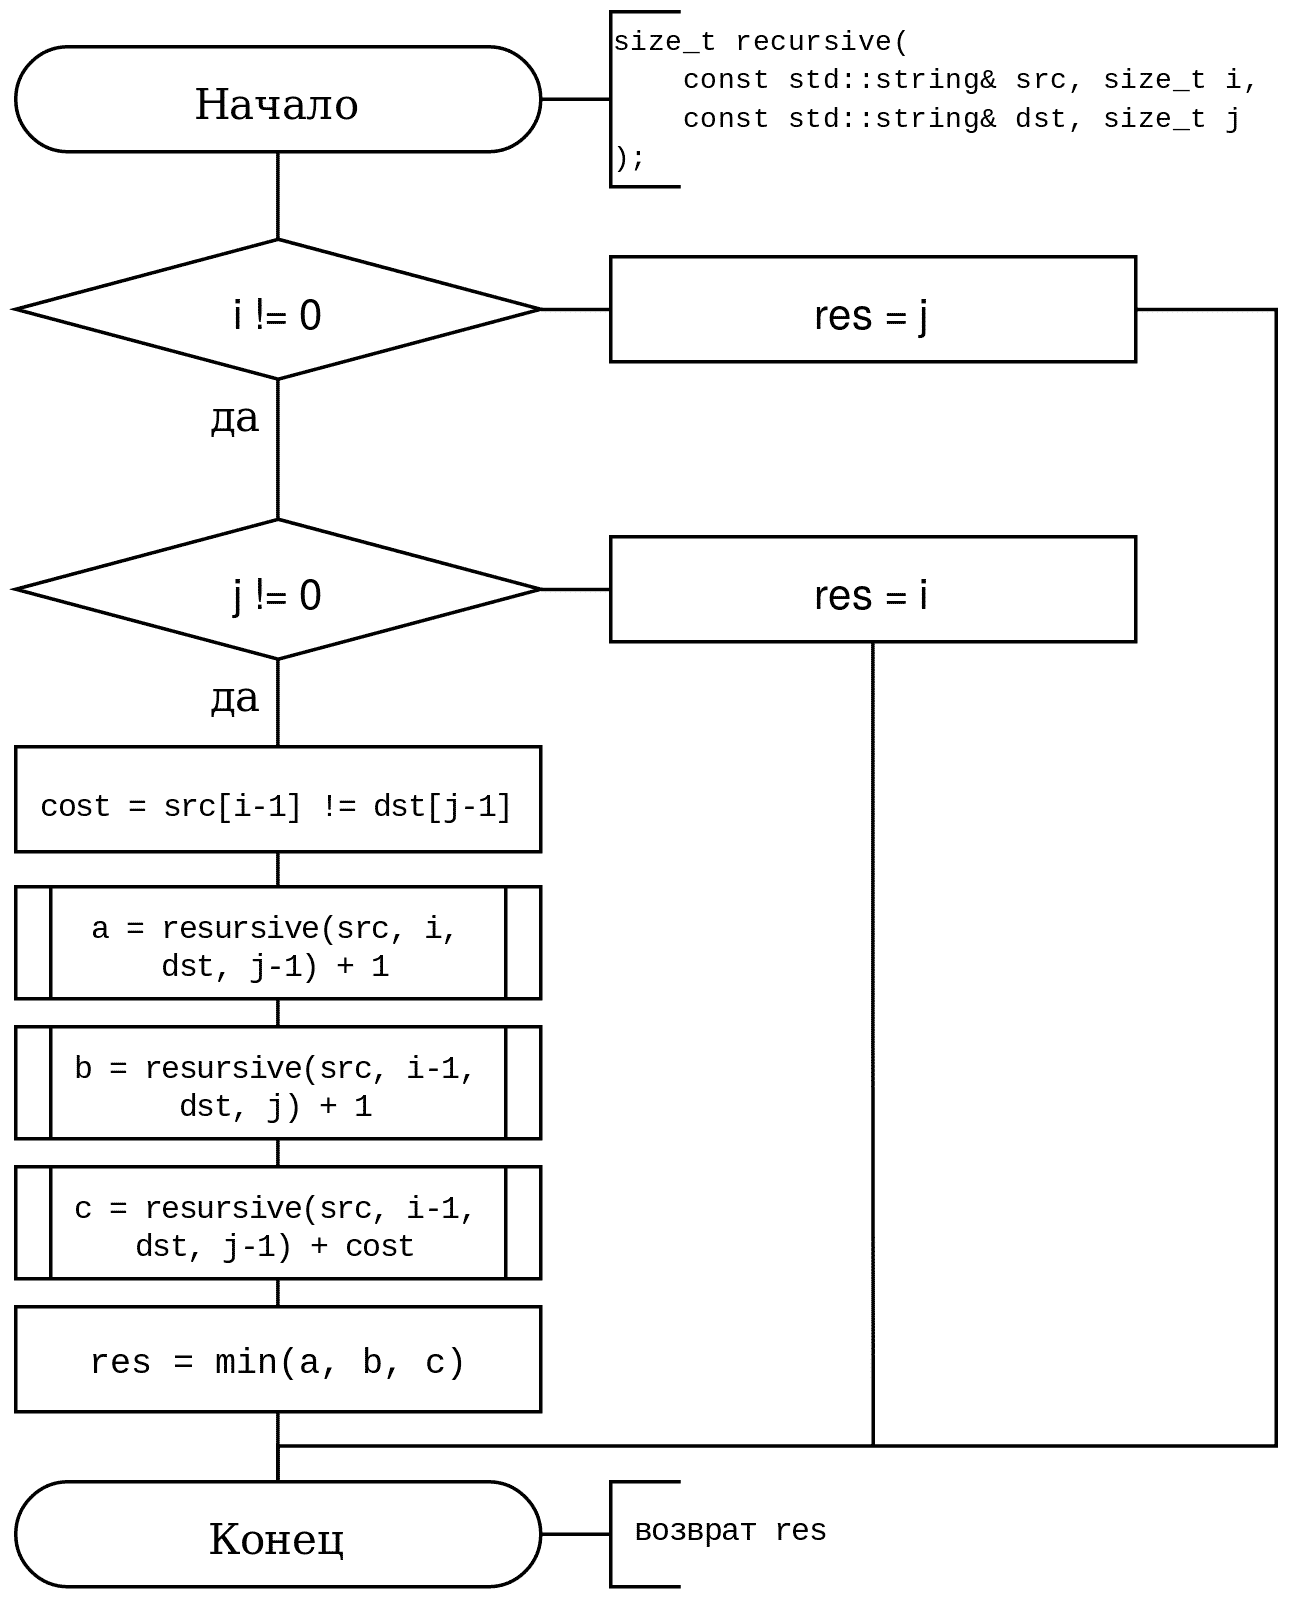
\includegraphics[height=190mm]{inc/img/levenshtein_detail_recursive}}
	\caption{Схема рекурсивного алгоритма Левенштейна}
	\label{img:levenshtein_recursive}
\end{figure}

\img{250mm}{levenshtein_damerau}{Схема итеративного алгоритма Дамерау — Левенштейна}
